%%%%%%%%%%%%%%%%%%%%%%%%%%%%%%%%%%%%%%%%%%%%%%%%%%%%%%%%%%%%%%%%%%%%%%

%
%%%%%%%%%%%%%%%%%%%%%%%%%%%%%%%%%%%%%%%%%%%%%%%%%%%%%%%%%%%%%%%%%%%%%%

\documentclass[10pt,landscape]{article}
\usepackage{amssymb,amsmath,amsthm,amsfonts}
\usepackage{multicol,multirow}
\usepackage{enumitem}
\usepackage{calc}
\usepackage{ifthen}
\usepackage[landscape]{geometry}
\usepackage[colorlinks=true,citecolor=blue,linkcolor=blue]{hyperref}
\usepackage{pdfpages}


\ifthenelse{\lengthtest { \paperwidth = 11in}}
    { \geometry{top=.5in,left=.5in,right=.5in,bottom=.5in} }
	{\ifthenelse{ \lengthtest{ \paperwidth = 297mm}}
		{\geometry{top=1cm,left=1cm,right=1cm,bottom=1cm} }
		{\geometry{top=1cm,left=1cm,right=1cm,bottom=1cm} }
	}
\pagestyle{empty}
\makeatletter
\renewcommand{\section}{\@startsection{section}{1}{0mm}%
                                {-1ex plus -.5ex minus -.2ex}%
                                {0.5ex plus .2ex}%x
                                {\normalfont\large\bfseries}}
\renewcommand{\subsection}{\@startsection{subsection}{2}{0mm}%
                                {-1explus -.5ex minus -.2ex}%
                                {0.5ex plus .2ex}%
                                {\normalfont\normalsize\bfseries}}
\renewcommand{\subsubsection}{\@startsection{subsubsection}{3}{0mm}%
                                {-1ex plus -.5ex minus -.2ex}%
                                {1ex plus .2ex}%
                                {\normalfont\small\bfseries}}
                                
\newcommand\todo[1]{\textcolor{red}{#1}}

\makeatother
\setcounter{secnumdepth}{0}
\setlength{\parindent}{0pt}
\setlength{\parskip}{0pt plus 0.5ex}

\theoremstyle{definition}
\newtheorem*{question}{Question}
\newtheorem*{method}{Method}
\newtheorem{theorem}{Theorem}
\newtheorem{defin}{Definition}
\newtheorem{type}{Type}
\theoremstyle{remark}
\newtheorem*{remark}{Remark}


% -----------------------------------------------------------------------

\title{Cheatsheet}

\begin{document}

\raggedright
\footnotesize

\begin{center}
     \Large{\textbf{MATH 257 Cheatsheet with \LaTeX}} \\
\end{center}
\begin{multicols}{3}
\setlength{\premulticols}{1pt}
\setlength{\postmulticols}{1pt}
\setlength{\multicolsep}{1pt}
\setlength{\columnsep}{2pt}

%%%%%%%%%%%%%%%%%%%%%%%%%%%%%%%%%%%%%%%%%%%%%%%%%%%%%%%%%%%%%
% for no space list, use [noitemsep,nolistsep]. It ony works for itemsize.

%%%%%%%%%%%%%%%%%%%%%%%%%%%%%%%%%%%%%%%%%%%%%%%%%%%%%%%%%%%%%
%%%%%%%%%%%%%%%%%%%%%%%%%% section %%%%%%%%%%%%%%%%%%%%%%%%%%
%%%%%%%%%%%%%%%%%%%%%%%%%%%%%%%%%%%%%%%%%%%%%%%%%%%%%%%%%%%%%
\section{Basics}
\subsection{Solve 1st order ODE}

\subsection{Solve 2nd order ODE}

\subsubsection{Special Case}
\textbf{Cauchy-Euler/Eqidimensional}: $$x^2y''+axy'+by=0$$  \\
use $y = x^r$ to solve. 

%%%%%%%%%%%%%%%%%%%%%%%%%%%%%%%%%%%%%%%%%%%%%%%%%%%%%%%%%%%%%
%%%%%%%%%%%%%%%%%%%%%%%%%% section %%%%%%%%%%%%%%%%%%%%%%%%%%
%%%%%%%%%%%%%%%%%%%%%%%%%%%%%%%%%%%%%%%%%%%%%%%%%%%%%%%%%%%%%
\section{Series solution}
\textbf{Power Series}: $f(x) = \sum^{\infty}_{i=0}a_ix^i$ \\
\textbf{Talyor Series}: condition on power series that series is continuous and infinitely differentiable. $f(x) = \sum^{\infty}_{i=0} \frac{f^n(x_0)}{n!}(x-x_0)^n$ \\
\textbf{Maclaurin Series}: taylor series where $x_0 = 0$ $f(x) = \sum^{\infty}_{i=0} \frac{f^n(0)}{n!}(x)^n$ \\

\subsection{Convergence}
$|x-x_0| < P$, where P is the radius of convergnece. Use ratio test: $\lim_{i \rightarrow \infty} |\frac{Q_{i+1}}{Q_i}| < 1$

\textbf{Analytic}: T-series expansion exist at $x_)$, then the function is analytic at $x_0$ with the radius of convergence. 

\subsection{Singular point}
Take function $$\mathcal{L}y = P(x)y'' + Q(x)y' + R(x)y = 0$$ 
Transform function to $$\mathcal{L}y = y'' + p(x)y' + q(x)y = 0$$ 
where $p(x)= \frac{Q(x)}{P(x)}$ and $q(x)= \frac{R(x)}{P(x)}$. if p(x) or q(x) does not converge at $x_0$, there is a SP at $x_0$(Also not analytic)  \\

\textbf{Regular Singular Point (RSP)}: \\
Transform function to $$\mathcal{L}y = (x-x_0)^2y'' + \alpha(x) (x-x_0)y' + \beta(x)y = 0$$ where $\alpha(x) = \frac{Q(x)}{P(x)}(x-x_0)$, $\beta(x) = \frac{R(x)}{P(x)}(x-x_0)^2$. if $lim_{x\rightarrow x_0} \alpha(x) = c_1$ and $lim_{x\rightarrow x_0} \beta(x) = c_2$, then $x_0$ is RSP. Other wise it's an Iregular Singuar point(IRSP).


\subsubsection{Solve RP}
\textbf{Frobenius Series}: $f(x) = (x-x_0)^r\sum^{\infty}_{i=0}a_i(x-x_0)^i$ \\



%%%%%%%%%%%%%%%%%%%%%%%%%%%%%%%%%%%%%%%%%%%%%%%%%%%%%%%%%%%%%
%%%%%%%%%%%%%%%%%%%%%%%%%% section %%%%%%%%%%%%%%%%%%%%%%%%%%
%%%%%%%%%%%%%%%%%%%%%%%%%%%%%%%%%%%%%%%%%%%%%%%%%%%%%%%%%%%%%
\section{PDE solving Methods}

\subsection{Boundary Condition}
\begin{itemize} [noitemsep,nolistsep]
    \item \textbf{Dirichlet:} 
    \begin{itemize}
        \item Heat: $u(0,t) = u(L,t)= 0$ 
        \item Laplace: 
            $\begin{cases}
                \text{finite}: \\
                \text{semi-infinite strip}:\\
            \end{cases}$
    \end{itemize}
    
    \item \textbf{Neumann:} $u_x (0,t) = u_x (L, t) = 0$ 
    
    \item \textbf{Periodic:} 
        \begin{itemize}
            \item Heat:         
                $\begin{cases}
                u(0,t) = u(L,t) \\
                u_x(0,t) = u_x(L,t) \\
                \end{cases}$
            \item Wave
            \item Laplace
        \end{itemize}
        

    \item \textbf{Mixed type A:} 
        $\begin{cases}
        u(0,t) = u_x(L,t) = 0 \\
        u(x,0) = f(x) \\
        \end{cases}$
    \item \textbf{Mixed type B:} 
        $\begin{cases}
        u_x(0,t) = u(L,t) = 0 \\
        u(x,0) = f(x) \\
        \end{cases}$
\end{itemize}


%%%%%%%%%%%%%%%%%%%%%%%%%%%%%%%%%%%%%%%%%%%%%%%%%%%%%%%%%%%%%
%%%%%%%%%%%%%%%%%%%%%%%%%% section %%%%%%%%%%%%%%%%%%%%%%%%%%
%%%%%%%%%%%%%%%%%%%%%%%%%%%%%%%%%%%%%%%%%%%%%%%%%%%%%%%%%%%%%
\section{Laplace's Equation}
\textbf{Special steady state of Wave or Heat equations where there is no time invariant: $\frac{\partial u}{\partial t} = \frac{\partial u^2}{\partial^2 t} = 0$}
$$\Delta u = \frac{\partial u^2}{\partial^2 t} + \frac{\partial u^2}{\partial^2 x}  = 0$$

\subsection{Types}
\textbf{Infinite Bound}
Let u(x) = w(x, t) + v(x). Solve for both with the usual way. 

\subsubsection{Circle}
 Laplace: Transform to polar coordinate \\
$u_{xx} + u_{yy} = U_{rr} + \cfrac{1}{r}U_r + \cfrac{1}{r^2}U_{\theta \theta} = 0$\\
where 
$\begin{cases}
r = (x^2+y^2)^\frac{1}{2} \\
\theta = atan(\frac{y}{x})\\
\end{cases}$


\subsubsection{Wedge}
\textbf{characteristics}: $u_{xx} + u_{yy} = U_{rr} + \cfrac{1}{r}U_r + \cfrac{1}{r^2}U_{\theta \theta} = 0$, where $0 < r < a$, $0< \theta < \alpha$ \\
\begin{itemize}[noitemsep,nolistsep]
    \item $u(r,0)=c_1, \; u(r, \alpha) = c_2$, $u(r, \theta)$ bounded as $r \rightarrow 0, u(\alpha, \theta) = f(\theta)$ 
    \item $u_{\theta}(r,0)=c_1, \; u_{\theta}(r, \alpha) = c_2$, $u(r, \theta)$ bounded as $r \rightarrow 0, u(\alpha, \theta) = f(\theta)$ 
    \item $u_{\theta}(r,0)=c_1, \; u(r, \alpha) = c_2$, $u(r, \theta)$ bounded as $r \rightarrow 0, u(\alpha, \theta) = f(\theta)$ 
    \item Neumann on the interior of circle: $u_r(a, \theta) = f(\theta)$, as $r \rightarrow \infty, \; u(r, \theta) < \infty$ and periodic: $u(r, \theta) = u(r, \theta + 2\pi)$
\end{itemize}
\subsubsection{Special types}


\begin{itemize}[noitemsep,nolistsep]
    \item Wedge with hole: on top of wedge, some edge $u(b, \theta)$ is also defined.  $u(r,0)=c_1, \; u(r, \alpha) = c_2 \; u(b, \theta) = 0$, $u(r, \theta)$ bounded as $r \rightarrow 0, u(\alpha, \theta) = f(\theta)$  
    \begin{method}
    
    \end{method}
    
    \item Dirichlet on the interior of circle: $u(a, \theta) = f(\theta)$, as $r \rightarrow 0, \; u(r, \theta) < \infty$ and periodic: $u(r, \theta) = u(r, \theta + 2\pi)$
    \item Dirichlet on the exterior of circle: $u(a, \theta) = f(\theta)$, as $r \rightarrow \infty, \; u(r, \theta) < \infty$ and periodic: $u(r, \theta) = u(r, \theta + 2\pi)$
\end{itemize}

\todo{Possion integral forma}

%%%%%%%%%%%%%%%%%%%%%%%%%%%%%%%%%%%%%%%%%%%%%%%%%%%%%%%%%%%%%
%%%%%%%%%%%%%%%%%%%%%%%%%% section %%%%%%%%%%%%%%%%%%%%%%%%%%
%%%%%%%%%%%%%%%%%%%%%%%%%%%%%%%%%%%%%%%%%%%%%%%%%%%%%%%%%%%%%

\section{Strum-Louisville Boundary Value Problem}
\begin{defin}
Boundary value problem of the form:
$$(p(x)y')' - q(x)y + \lambda r(x)y = 0\; 0 < x < \ell$$ \\
$$\alpha_1 y(0) + \alpha_2 y'(0) = 0 \; \beta_1 y(\ell) + \beta_2 y'(\ell) = 0$$  \\
where $p, p', q, r$ are continuous on $0 \leq x \leq \ell $ and $p(x) \geq 0$ and $r(x) >0 $ on $0 \leq x \leq \ell $ \\
Then Strum-Liouville eigenvalue problem: \\
$$\mathcal{L} = \lambda ry = -(py')' + qy$$
$$\alpha_1 y(0) + \alpha_2 y'(0) = 0 \; \beta_1 y(\ell) + \beta_2 y'(\ell) = 0$$
$$p(x) > 0, r(x) >0$$
\end{defin}
find $\mu = \frac{e^{\int \frac{Q}{P}}}{P}$

\textbf{Properties}
\begin{itemize} [noitemsep,nolistsep]
    \item $\int^{\ell}_0 r(x) \phi^2_j (x) \mathrm{d}x = 1$
    \item if $f(x) = \sum^{\infty}_{n=1}c_n\phi_n(x)$, then 
    $$c_n = \frac{\int^b_af(x)\phi_n(x)r(x)dx}{\int^b_a\phi^2_n(x)r(x)dx}$$
\end{itemize}

\begin{question}
\begin{itemize}
    \item Ask for transform equations to S-L form. Compute all eigenvalue and eigenfunctions.
    \item USe the above to solve another PDE system. 
\end{itemize}

\end{question}

\subsection{Robin Boundary Condition}
\begin{align*}
    X'' + \lambda X &= 0
    \\ X'(0) &= h_1X(0), 
    \\ X'(\ell) &= -h_2X(\ell), \; h_z \geq 0, \; h_2 \geq 0
    \\ X(x) &= A \cos \mu x + B \sin \mu x, \; 
    \\ X'(x) &= - A \mu \sin\mu x + B \mu \cos\mu x
\end{align*}
Solve for $\tan(\mu\ell) = [\frac{\mu(h_1+h_2)}{\mu^2-h_1h_2}]$
\begin{itemize} [noitemsep,nolistsep]
    \item $h_1$, $h_2 \neq 0$ \\
    $$X_n = \frac{\mu_n}{h_1}\cos\mu_{n}x + \sin\mu_{n}x, \; \mu_n \rightarrow \frac{n\pi}{\ell} \; as \; n \rightarrow \infty$$
    \item $h_1 \neq 0$, $h_2 = 0$
    $$X_n = \frac{\mu_n}{h_1}\cos\mu_{n}x + \sin\mu_{n}x = \frac{\cos\mu_{n}(\ell - x)}{\sin\mu_{n}x}$$
    \item $h_1 \rightarrow \infty$, $h_2 \neq 0$
    $$X_n = \sin\mu_{n}x, \; \mu_{n} \rightarrow [(\frac{2n+1}{2})\frac{\pi}{\ell}]$$
\end{itemize}

%%%%%%%%%%%%%%%%%%%%%%%%%%%%%%%%%%%%%%%%%%%%%%%%%%%%%%%%%%%%%
%%%%%%%%%%%%%%%%%%%%%%%%%% section %%%%%%%%%%%%%%%%%%%%%%%%%%
%%%%%%%%%%%%%%%%%%%%%%%%%%%%%%%%%%%%%%%%%%%%%%%%%%%%%%%%%%%%%


\section{Tools and Useful Equations}
\textbf{Cauchy-Euler/Eqidimensional}: 
$$x^2y''+axy'+by=0$$  \\

\textbf{Legendre Equation}: $$(1-x^2)y'' - 2xy' + \alpha(\alpha+1)y = 0$$ \\

\textbf{Bessel's Equation}: $$x^2y'' + xy' + (x^2-v^2)y = 0$$

%%%%%%%%%%%%%%%%%%%%%%%%%%%%%%%%%%%%%%%%%%%%%%%%%%%%%%%%%%%%%
%%%%%%%%%%%%%%%%%%%%%%%%%% section %%%%%%%%%%%%%%%%%%%%%%%%%%
%%%%%%%%%%%%%%%%%%%%%%%%%%%%%%%%%%%%%%%%%%%%%%%%%%%%%%%%%%%%%
\section{Miscs}

%%%%%%%%%%%%%%%%%%%%%%%%%%%%%%%%%%%%%%%%%%%%%%%%%%%%%%%%%%%%%
%%%%%%%%%%%%%%%%%%%%%%%%%% section %%%%%%%%%%%%%%%%%%%%%%%%%%
%%%%%%%%%%%%%%%%%%%%%%%%%%%%%%%%%%%%%%%%%%%%%%%%%%%%%%%%%%%%%


\end{multicols}

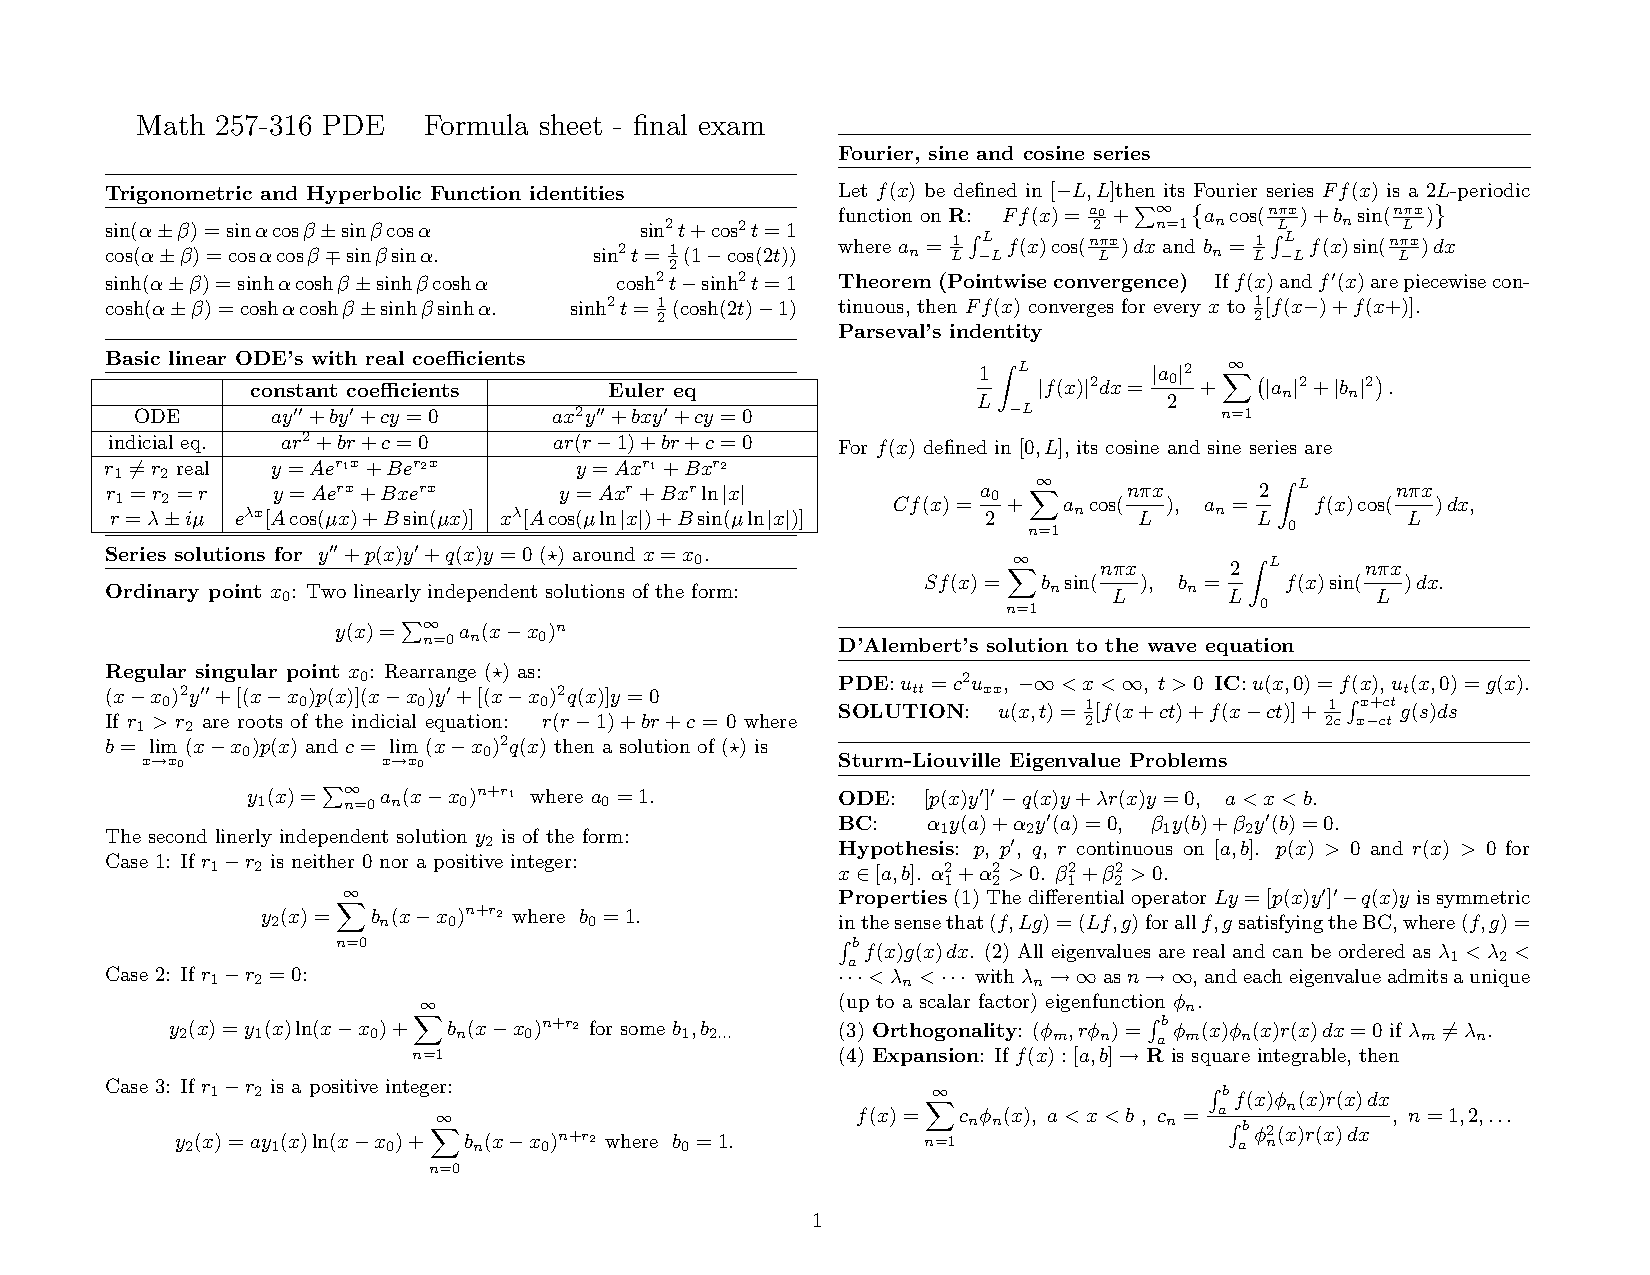
\includepdf{fs-final-reduced}

\end{document}
